\subsection{Rotational Invariance}\label{ex:rotation}
This example shows that if $\qoiA$ is defined by a rotation of $\qoiB$, then the accuracy and convergence rates of $\PP^{(a)}_{\pspace, \ndiscs, \nsamps}$ are identical to $\PP^{(b)}_{\pspace, \ndiscs, \nsamps}$.
We expect this to be true since skewness is rotationally invariant, as we summarize in the following Proposition.
\begin{prop}
The quantity $S_\qoi(\param)$ is invariant under rotations performed on $\qoi$ for any $\param$. \\
\label{prop:rot_invariance}
\end{prop}
\begin{proof}
If we apply a rotation $\qoi$, then the Jacobians $J_{\qoi, \param}$ are also subject to the same rotation at each $\param$.
Since rotations are unitary operators, the norms given in Eq.~\eqref{eq:skewness} used to define skewness are unaffected.
\end{proof}

\begin{figure}
\begin{minipage}{.5\textwidth}
\begin{table}[H]
\begin{tabular}{ c | c | c | c }
\nsamps & $\qoiA$ & $\qoiB$ & $\qoiC$\\ \hline \hline
$200$ & $2.18E-01$ & $1.97E-01$ & $2.19E-01$\\ \hline

$400$ & $1.60E-01$ & $1.70E-01$ & $1.51E-01$\\ \hline

$800$ & $1.09E-01$ & $1.14E-01$ & $1.09E-01$\\ \hline

$1600$ & $7.43E-02$ & $7.76E-02$ & $7.53E-02$\\ \hline

$3200$ & $5.51E-02$ & $5.53E-02$ & $5.31E-02$\\ \hline

$6400$ & $4.19E-02$ & $4.09E-02$ & $4.19E-02$\\ \hline
\end{tabular}
\end{table}
\end{minipage}
\begin{minipage}{.45\textwidth}
		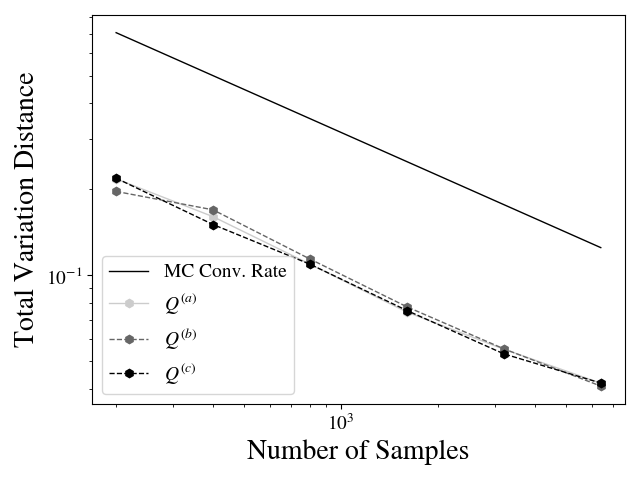
\includegraphics[width=\linewidth]{./images/Plot-orth-reg_BigN_40000_reg_M_1_rand_I_100000.png}
\end{minipage}
\caption{The results of $d^2_\text{TV}(\PP_{\pspace, \ndiscs, \nsamps}, \PP_{\pspace, \bar{\nsamps}})$ for three maps generated by random rotations of orthogonal linear maps.}
\label{fig:M1orth}
\end{figure}

To demonstrate this Lemma numerically, we define the space of QoI maps $\qspace = \set{ \qoiA , \qoiB, \qoiC }$, where all three are linear maps with the same local skewness $S_\qoi (\param) = 1 \; \forall \param \in \pspace$.
The map $\qoiA$ is the identity and the other two, $\qoiB$ and $\qoiC$ are rotations of $\qoiA$ by randomly chosen angles.
Following the algorithmic outline above, we perform a convergence study to $\PP_{\pspace,\bar{\nsamps}}$ with results summarized in Figure~\ref{fig:M1orth}.
The convergence rates and expected errors in the SIPs associated with each of these maps are virtually indistinguishable.
In light of Proposition~\ref{prop:rot_invariance} and these numerical results, we conclude that the accuracy of the numerical solution to the SIP is invariant under rotations to the QoI map.

\FloatBarrier
